\chapter{Milky Way diffuse background study: denoising and inpainting}
\label{ch_inpainting}

% \markright{Milky Way diffuse background study: denoising and inpainting}

In order to extract a  diffuse emission, we want to remove the  point sources from the data. 
As our HSD algorithm is very close to the MCA algorithm~\citep{starck:sta04}, an idea is to mask the most intense sources and to modify our algorithm in order to interpolate through the gaps exactly as in the MCA-Inpainting algorithm~\citep{inpainting:abrial06}. 
This modified algorithm can be called MS-VSTS-Inpainting algorithm.

The problem can be reformulated as a convex constrained minimization problem:

\begin{equation}
\label{inp_eq34}
\begin{split}
\text{Arg} \min_{\mathbf{X}} \| \mathbf{ \Phi}^{T}\mathbf{X}\|_1,
\text{s.t.} \\ \: \left\{\begin{array}{c}\mathbf{X} \geqslant 0 , \\\forall (j,k)\in \mathcal{M},      (\mathbf{ \Phi}^{T}\Pi \mathbf{X})_j[k]=(\mathbf{ \Phi}^{T} \mathbf{Y})_j[k] , \end{array}\right. 
\end{split}
\end{equation}
where $\Pi$ is a binary mask ($1$ on valid data and $0$ on invalid data).

The iterative scheme can be adapted to cope with a binary mask, which gives:
\begin{eqnarray}
\tilde{\mathbf{X}} = P_{+}[\mathbf{ X}^{(n)} + \mathbf{ \Phi} P_{\mathcal{M}} \mathbf{ \Phi}^{T} \Pi (\mathbf{ Y} - \mathbf{ X}^{(n)})] , \\
\mathbf{X}^{(n+1)} = \mathbf{ \Phi} \text{ST}_{\lambda_n}[\mathbf{ \Phi}\tilde{\mathbf{X}}] .
\end{eqnarray}


The thresholding strategy has to be adapted. Indeed, for the impainting task we need to have a very large initial threshold in order to have a very smooth image in the beginning and to refine the details progressively. We chose an exponentially decreasing threshold:
\begin{equation}
\label{eq42}
\lambda_{n} = \lambda_{\max}  (2^{(\frac{N_{\max} - n}{N_{\max} - 1})} -1),n=1,2,\cdots,N_{\max} ,
\end{equation}
where $\lambda_{\max} = \max (\mathbf{\Phi}^{T}\mathbf{X})$.

\begin{algorithm}
\caption{MS-VST + IUWT Denoising + Inpainting}
\label{alg2}

\begin{algorithmic}[1]
\REQUIRE $\quad$ data $a_0:=\mathbf{Y}$, mask $\Pi$, number of iterations $N_{\max}$, threshold $\kappa$.\\
\underline{\emph{\textbf{Detection}}} \\
\FOR{$j=1$ to $J$}
\STATE Compute $a_j$ and $d_j$ using (\ref{eq27}).
\STATE Hard threshold $|d_j[k]|$ with threshold $\kappa \sigma_j$ and update $\mathcal{M}$.
\ENDFOR \\
\underline{\emph{\textbf{Estimation}}} \\
\STATE Initialize $\mathbf{X}^{(0)}=0$, $\lambda_{0} = \lambda_{\max}$.
\FOR{$n=0$ to $N_{\max}-1$}
\STATE $\tilde{\mathbf{X}}= P_{+}[\mathbf{ X}^{(n)} + \mathbf{ \Phi} P_{\mathcal{M}} \mathbf{ \Phi}^{T} \Pi(\mathbf{ Y} - \mathbf{ X}^{(n)})]$.
\STATE $\mathbf{X}^{(n+1)} = \mathbf{ \Phi}^\text{ST}_{\lambda_n}[\mathbf{ \Phi}^{T}\tilde{\mathbf{X}}]$.
\STATE $\lambda_{n+1} = \lambda_{\max}  (2^{(\frac{N_{\max} - (n+1)}{N_{\max} - 1})} -1)$
\ENDFOR
\STATE Get the estimate $\hat{\mathbf{\Lambda}} = \mathbf{X}^{(N_{\max})}$.

\end{algorithmic}
\end{algorithm}



\section*{Experiment}

We applied this method on simulated Fermi data where we masked the most luminous sources.

The results are on Figure~\ref{impainting}. The MS-VST + IUWT + Inpainting method (Algorithm~\ref{alg2}) interpolates the missing data very well. Indeed, the missing part can not be seen anymore in the inpainted map, which shows that the diffuse emission component  has been correctly reconstructed.


\begin{figure}[htb]
\centering{
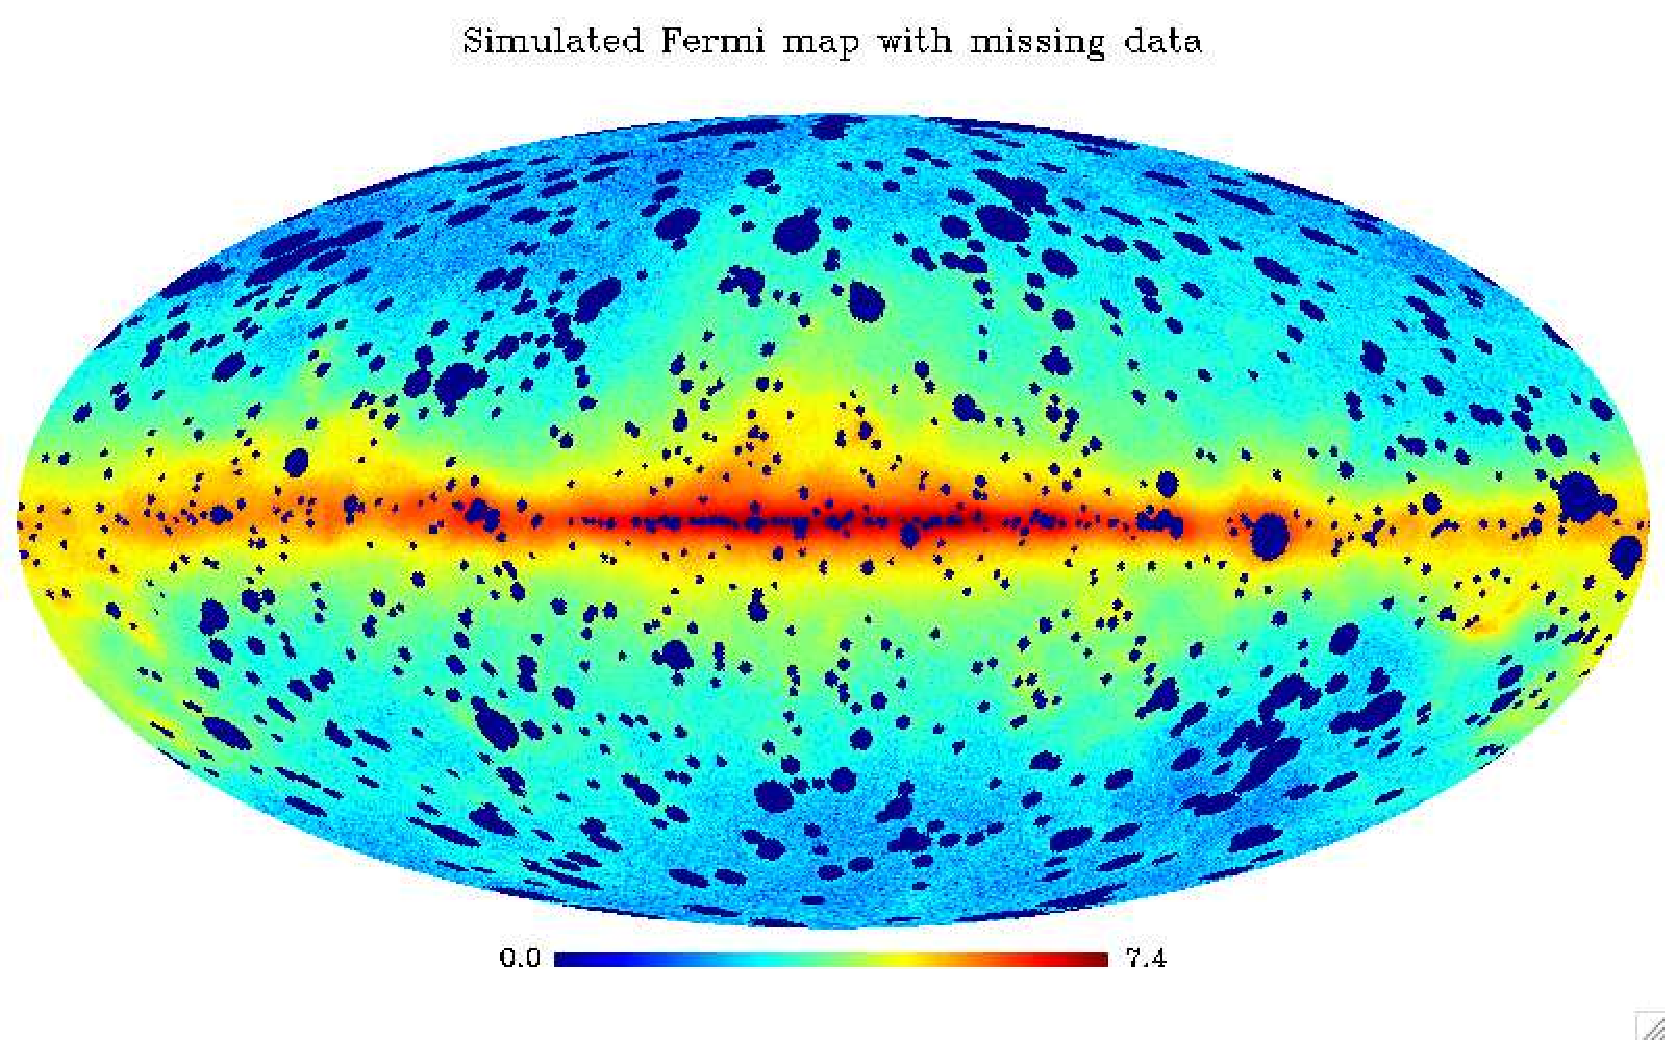
\includegraphics[width=5.5in]{13822fg22.pdf} 
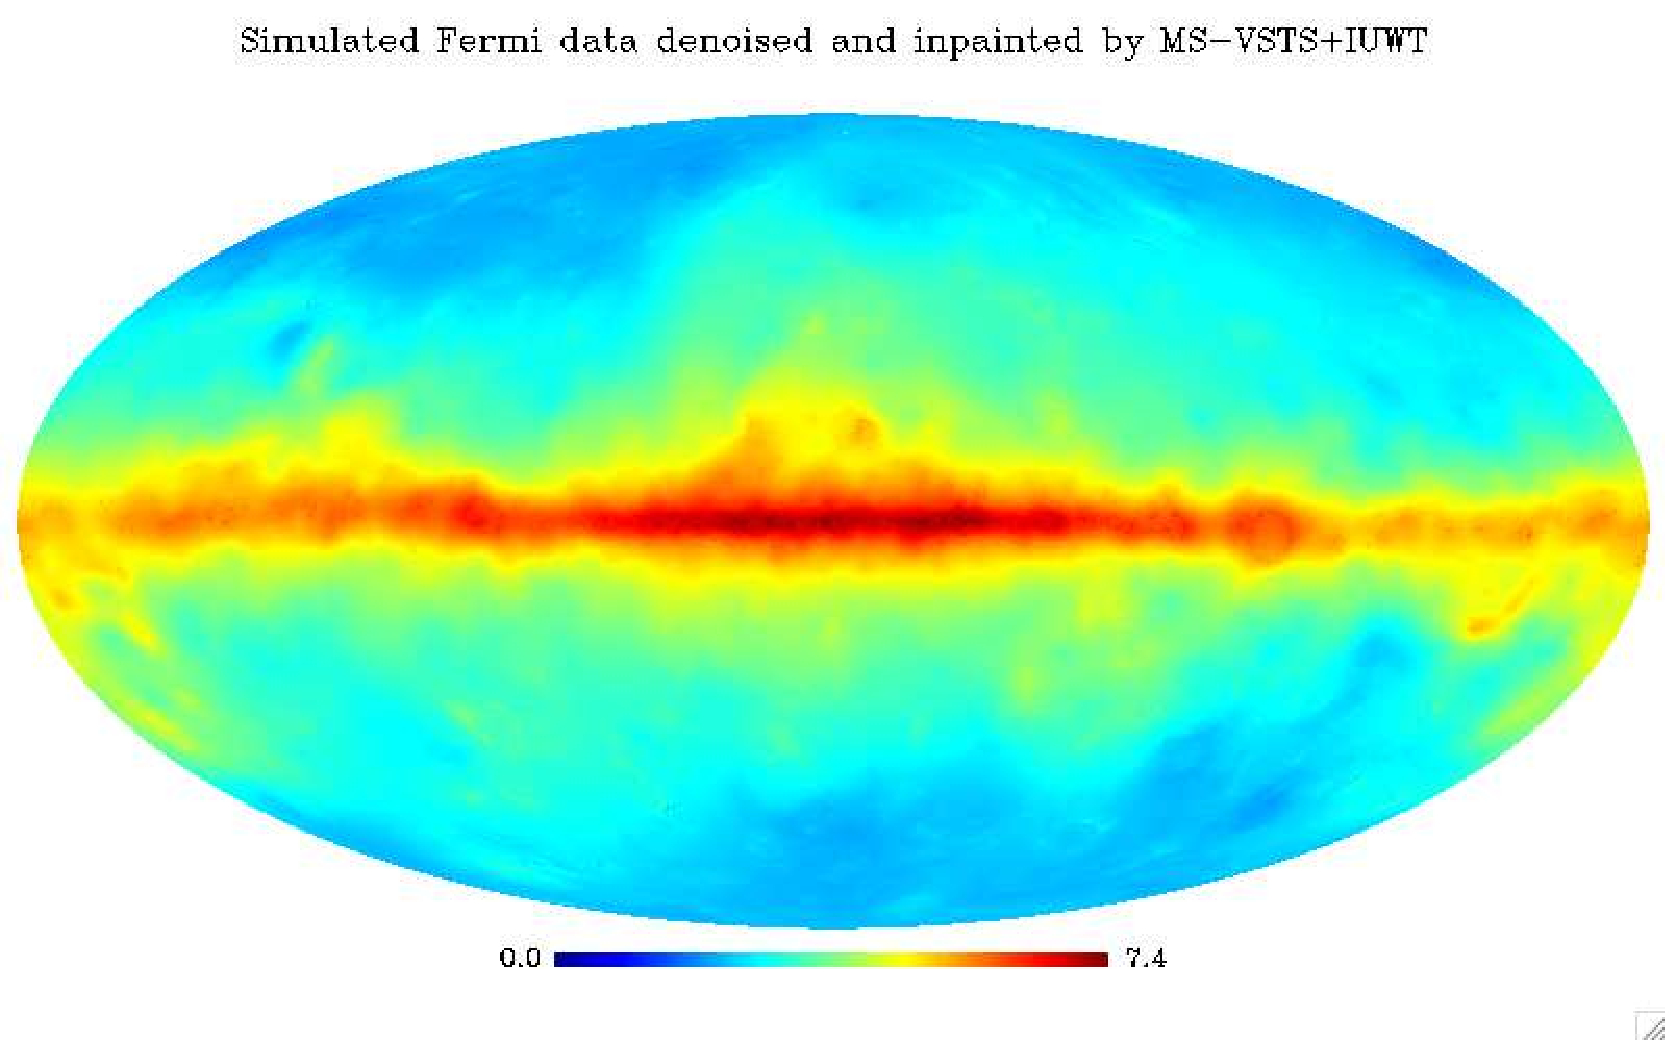
\includegraphics[width=5.5in]{13822fg23.pdf} 
}
\caption{MS-VSTS - Inpainting.
\emph{Top}: Fermi simulated map with Poisson noise and the most luminous sources masked.
\emph{Bottomt}: Fermi simulated map denoised and inpainted with wavelets (Algorithm~\ref{alg2}).
Pictures are in logarithmic scale.
}
\label{impainting}
\end{figure}
